\documentclass[
    pdftex,
    12pt,
    parskip=half,
    a4paper
]{scrartcl}
\author{Crawford, Sam}
\title{Netze und verteilte Systeme PS}

\usepackage[utf8]{inputenc}
\usepackage[naustrian]{babel}
\usepackage{graphicx}
\usepackage{xcolor}
\usepackage{listings}
\usepackage{subcaption}

\lstdefinestyle{cli}{
    backgroundcolor=\color{lightgray!20},   % lightgray background colour
    basicstyle=\ttfamily,                   % monospaced font
    frame=single,                           % sets a single-line border
    rulecolor=\color{gray!50},              % colour of the border
    belowskip=-2mm,                         % less vertical space after environment
    xleftmargin=1.5mm,                      % left padding
    xrightmargin=1.5mm                      % right padding
}
\lstset{style=cli}

\begin{document}
\section{Aufgabenstellung}
\textit{Übertragen Sie mindestens 10 Mal eine etwa 10 MB große Datei einmal mittels HTTP/1.1 bei
gleicher Empfangsgüte und noch einmal mit HTTP/1.1 vom gleichen Server (zB von Ihrem Cosy-
Webspace) zum Mess-Rechner bei schlechter werdendem Empfang und erstellen Sie von der
Übertragung mit tshark/tcpdump oder Wireshark ein Diagramm mit den Sequenznummern von TCP
auf der Y-Achse und der verstrichenen Zeit auf der X-Achse. Machen Sie dabei beide Messungen
im WLAN und beobachten/visualisieren/diskutieren/erklären Sie die Effekte bei der zweiten
Messung von schlechte(re)m Empfang zB durch immer größeren Abstand zum WLAN Access Point
(AP).
Beschreiben Sie möglichst genau den Messaufbau und verwendeten Geräte und Technologien!
Es sollen also 2 Messungen mit mindestens je 10 Diagrammen erstellt werden, die erste mit
Download bei gleichbleibender Empfangsgüte, die zweite bei schlechter werdendem Empfang (zB
größeren Abstand zum AP oder …).}

\vspace{3cm}%vspace

\begin{lstlisting}
$ ssh scrawford@141.201.2.44
$ fallocate --length 10M file
$ mv file	public_html
$ chmod a+r public_html/file
$ exit
\end{lstlisting}

\vspace{2cm}%vspace
\begin{lstlisting}
$ tcpdump --list-interfaces
\end{lstlisting}
\vspace{2cm}%vspace

\begin{lstlisting}
$ sudo tcpdump --interface wlo1 -w dump.pcap
\end{lstlisting}
\vspace{2cm}%vspace
\begin{lstlisting}
$ wget --delete-after \
       http://student.cosy.sbg.ac.at/~scrawford/file
\end{lstlisting}
\vspace{2cm}%vspace
\begin{lstlisting}
$ sudo killall tcpdump 
\end{lstlisting}

\vspace{2cm}%vspace
\begin{lstlisting}
$ wireshark dump.pcap
\end{lstlisting}
\vspace{4cm}%vspace

\begin{figure}
	\begin{subfigure}{0.5\textwidth}
		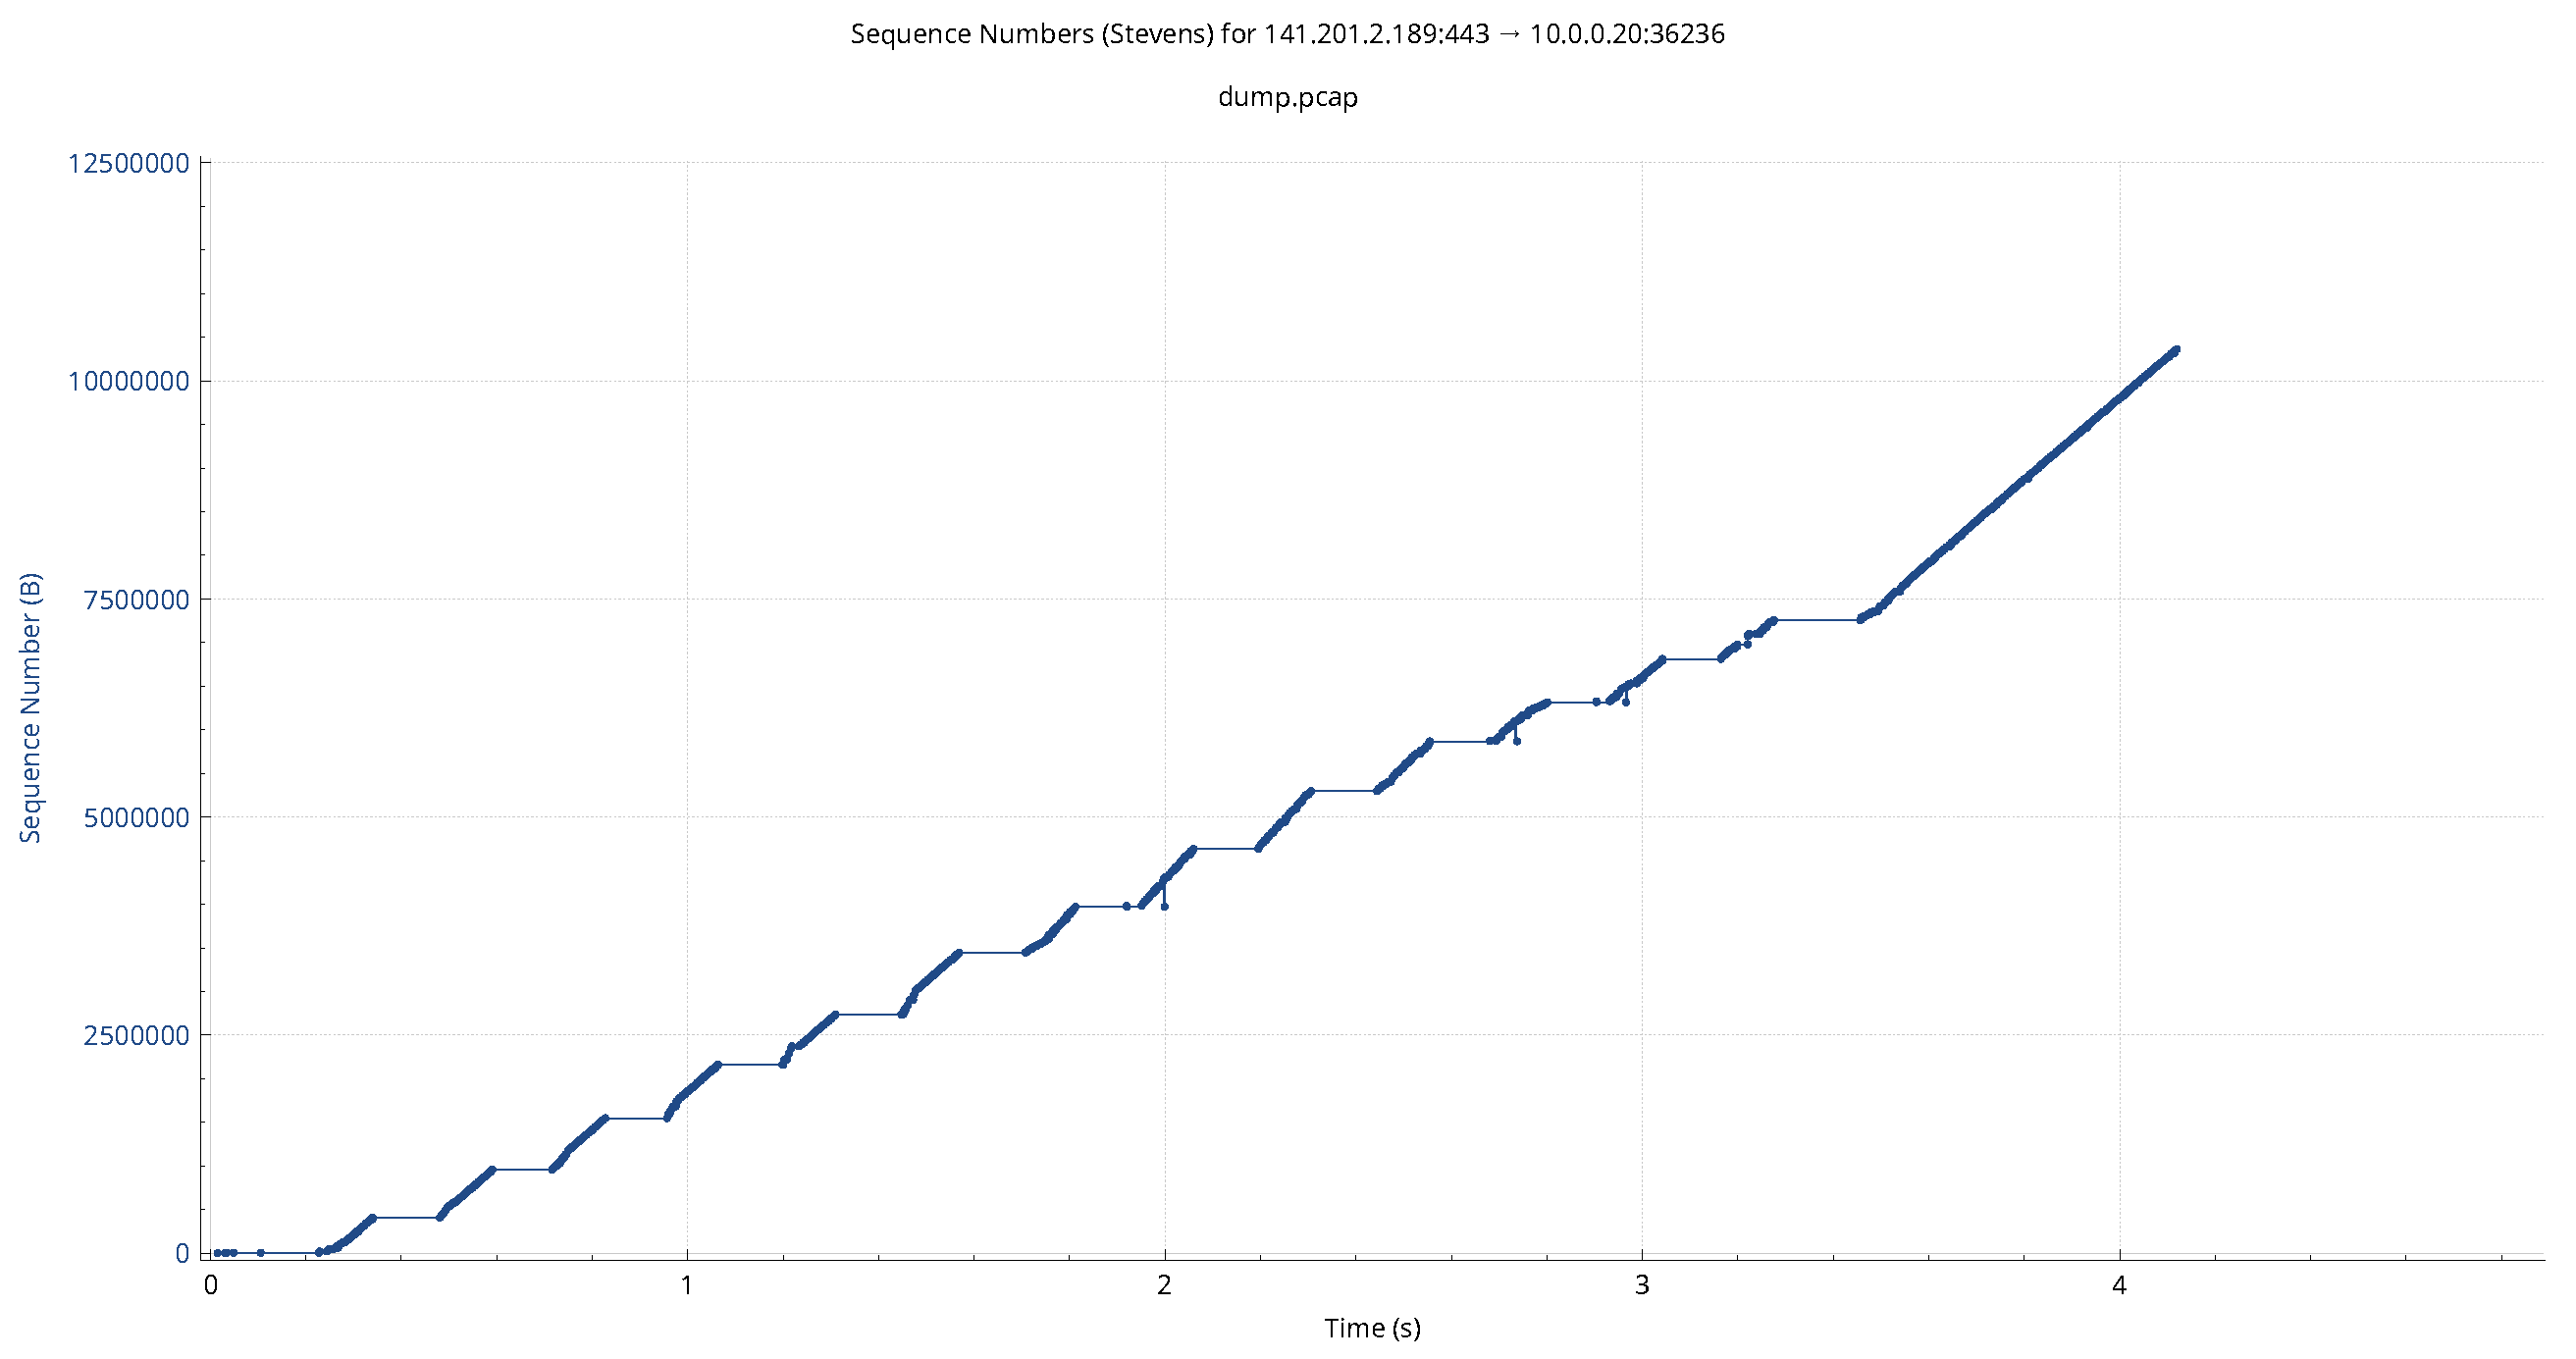
\includegraphics[width=1\textwidth]{../1/wireshark/constant1.pdf}
	\end{subfigure}
	\begin{subfigure}{0.5\textwidth}
		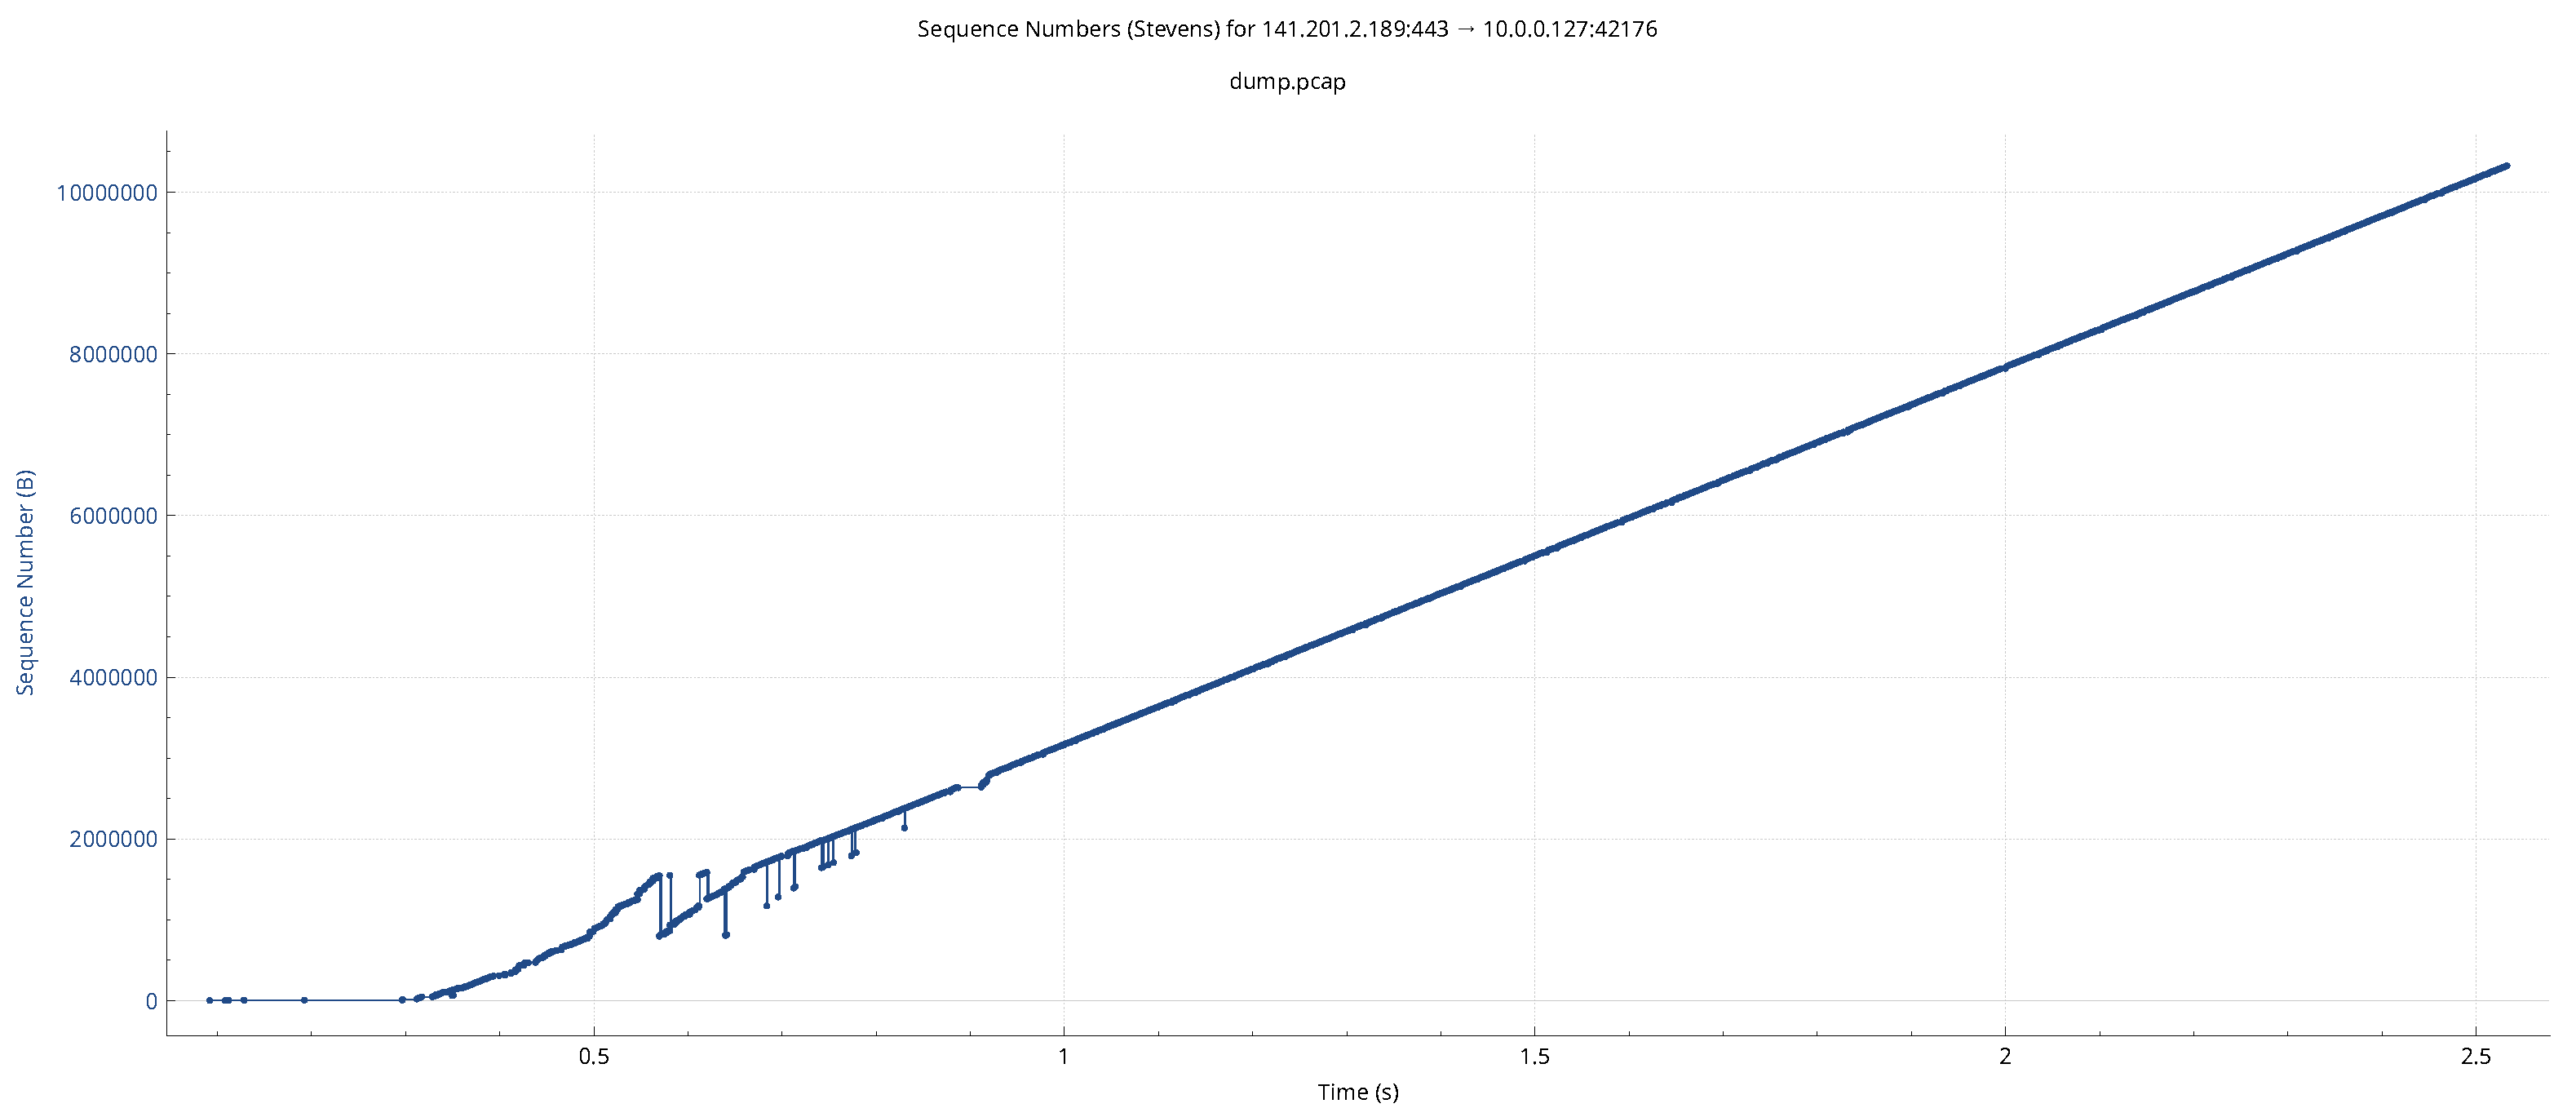
\includegraphics[width=1\textwidth]{../1/wireshark/constant2.pdf}
	\end{subfigure}
	\begin{subfigure}{0.5\textwidth}
		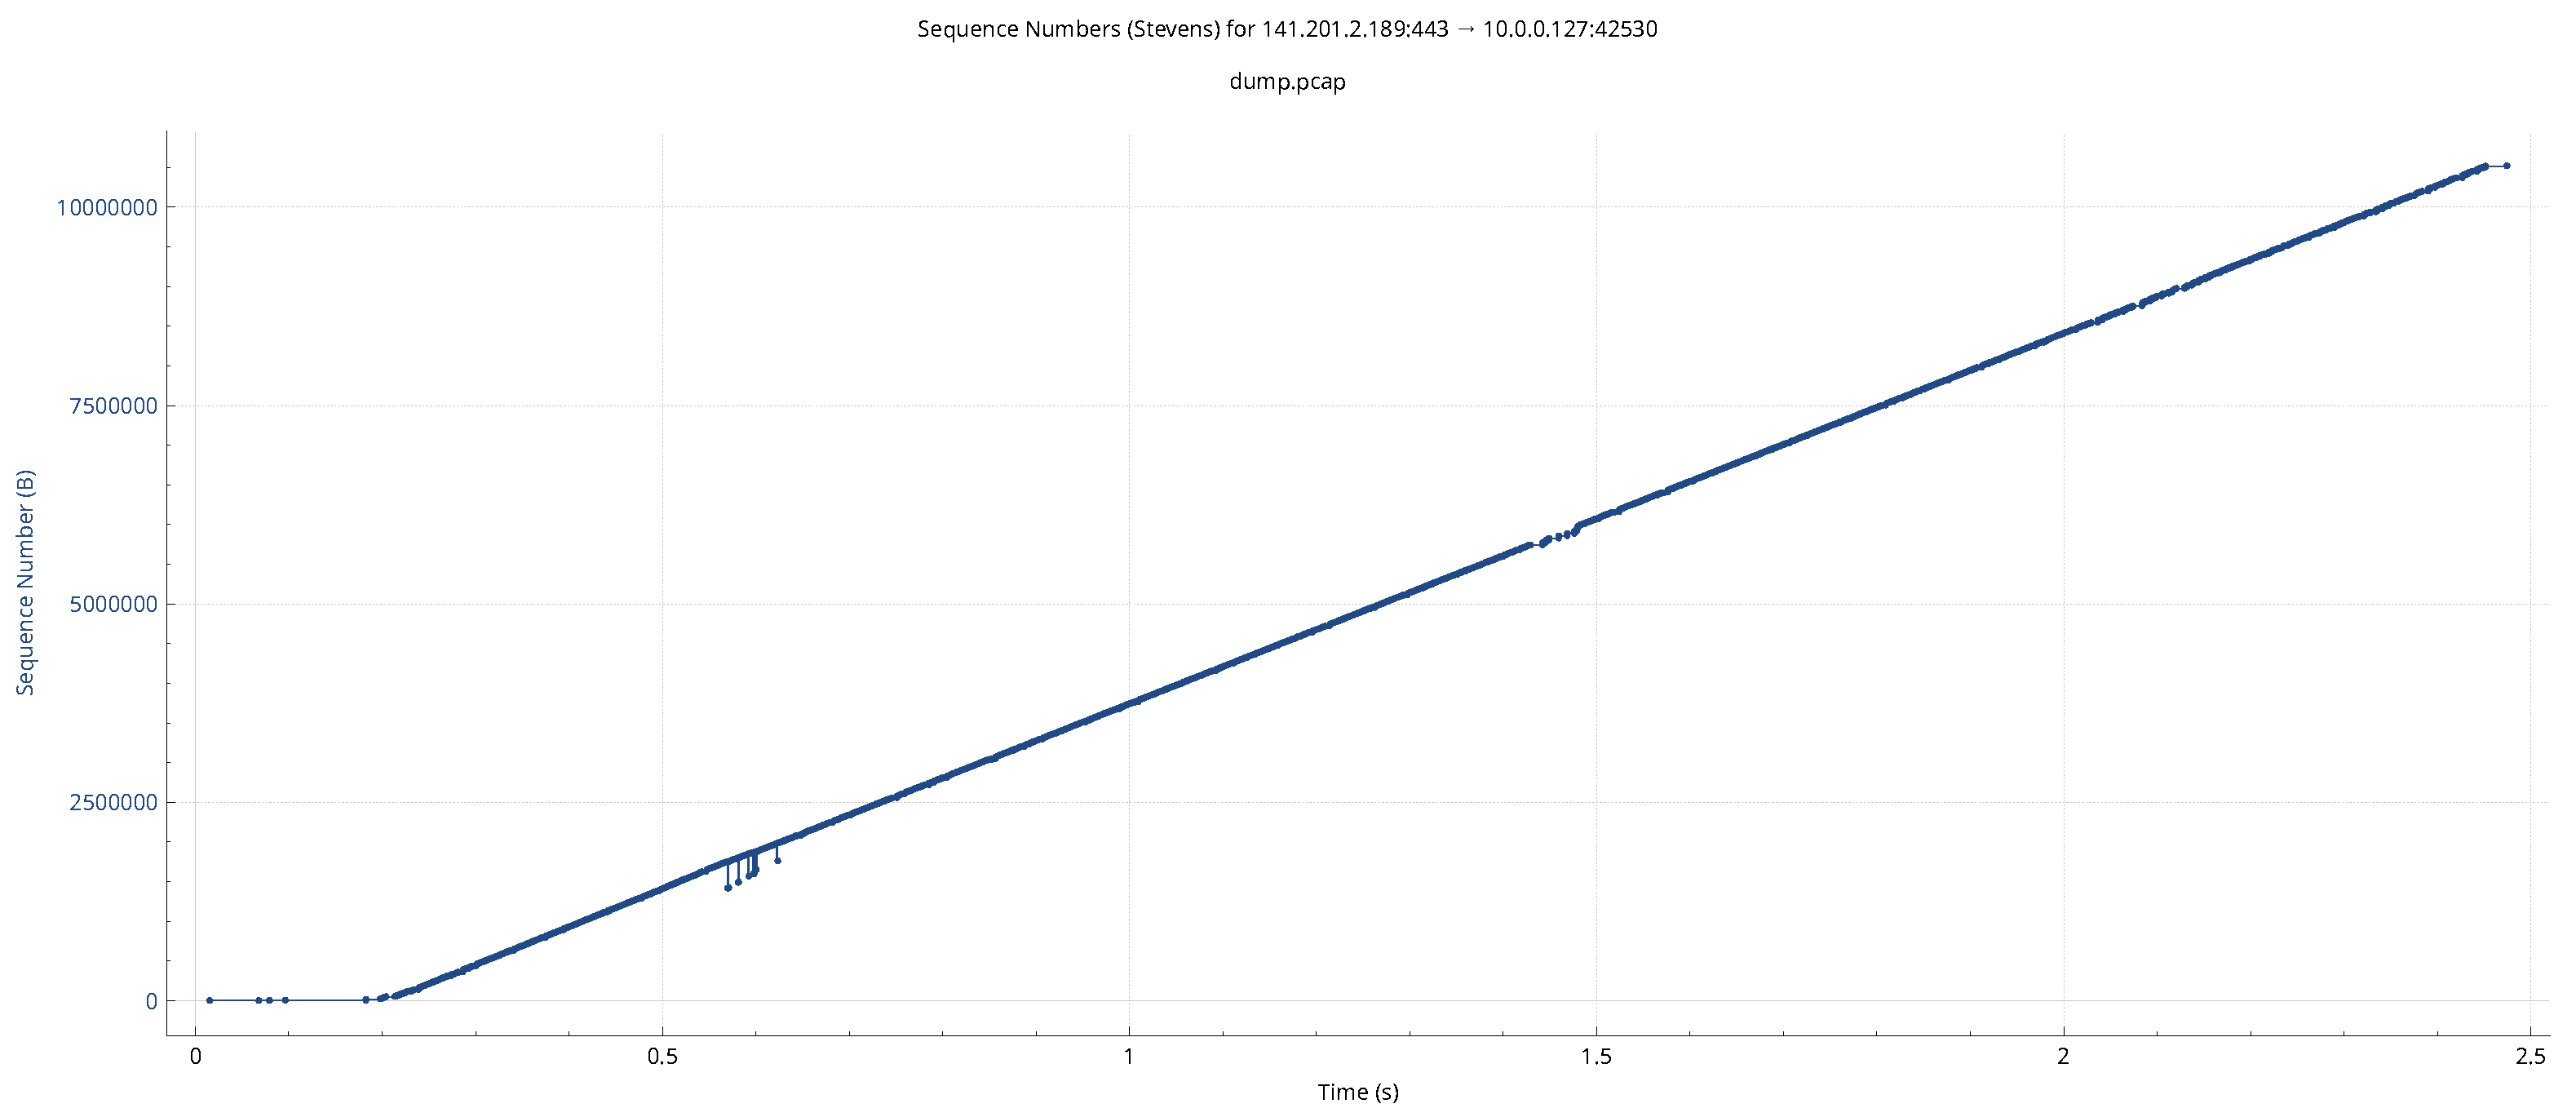
\includegraphics[width=1\textwidth]{../1/wireshark/constant3.pdf}
	\end{subfigure}
	\begin{subfigure}{0.5\textwidth}
		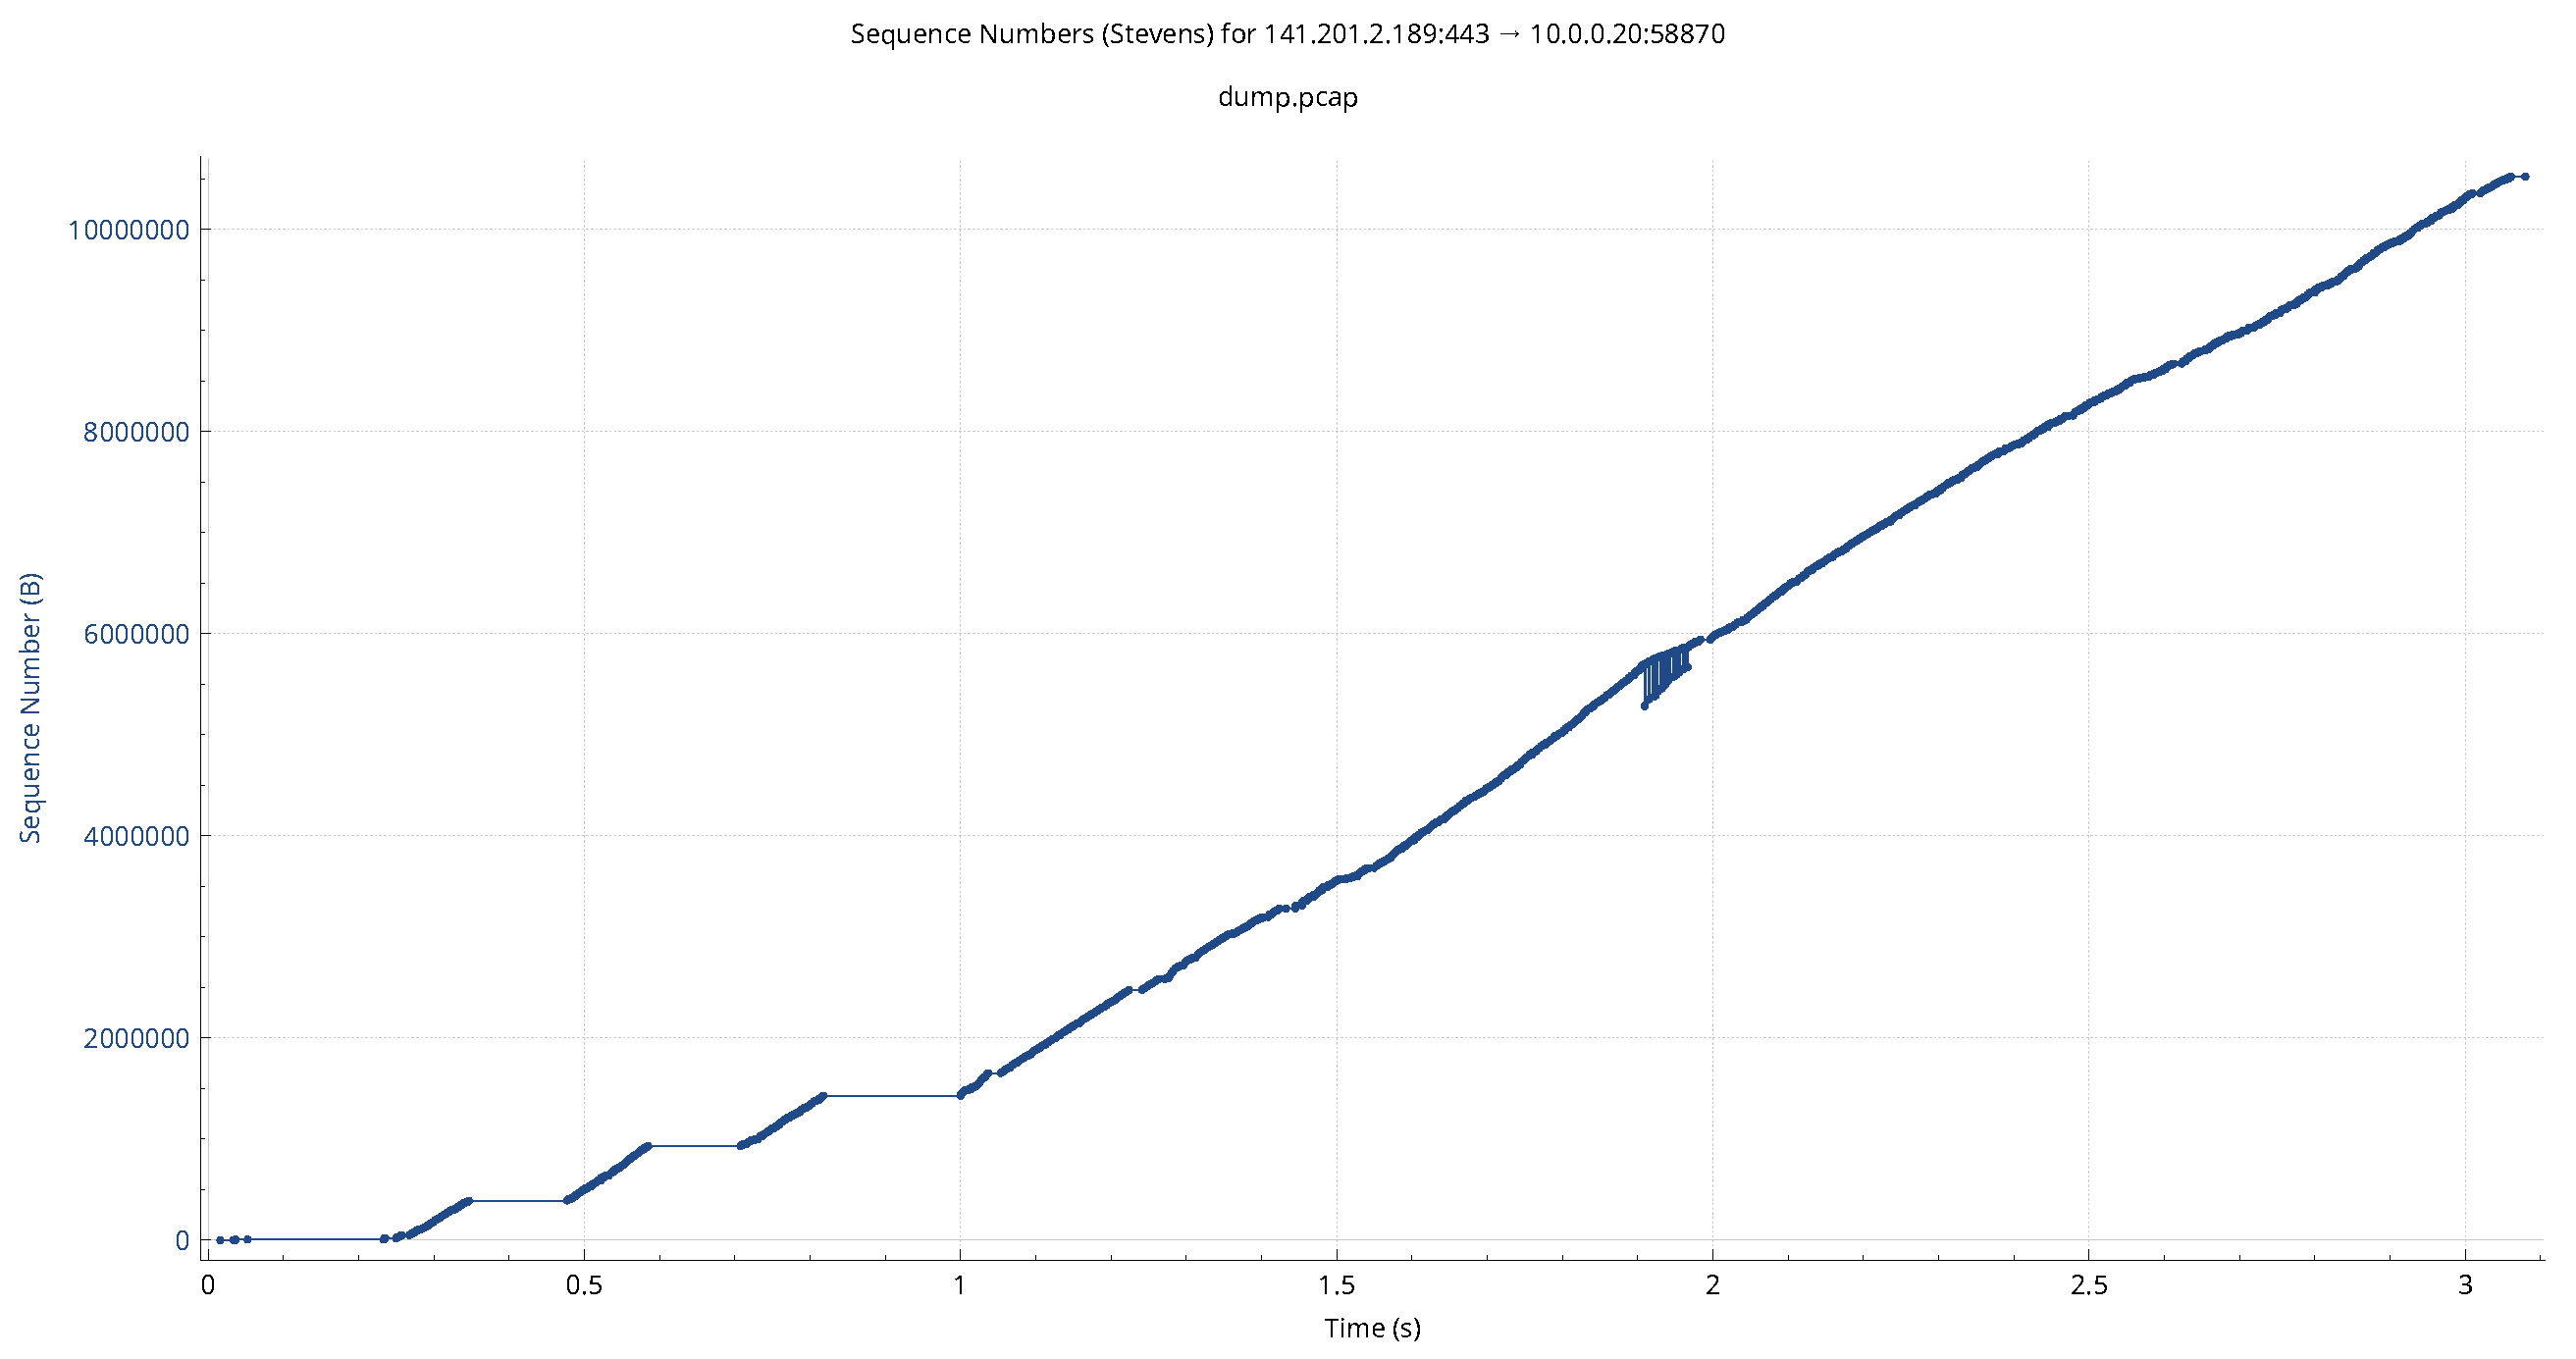
\includegraphics[width=1\textwidth]{../1/wireshark/constant4.pdf}
	\end{subfigure}
	\begin{subfigure}{0.5\textwidth}
		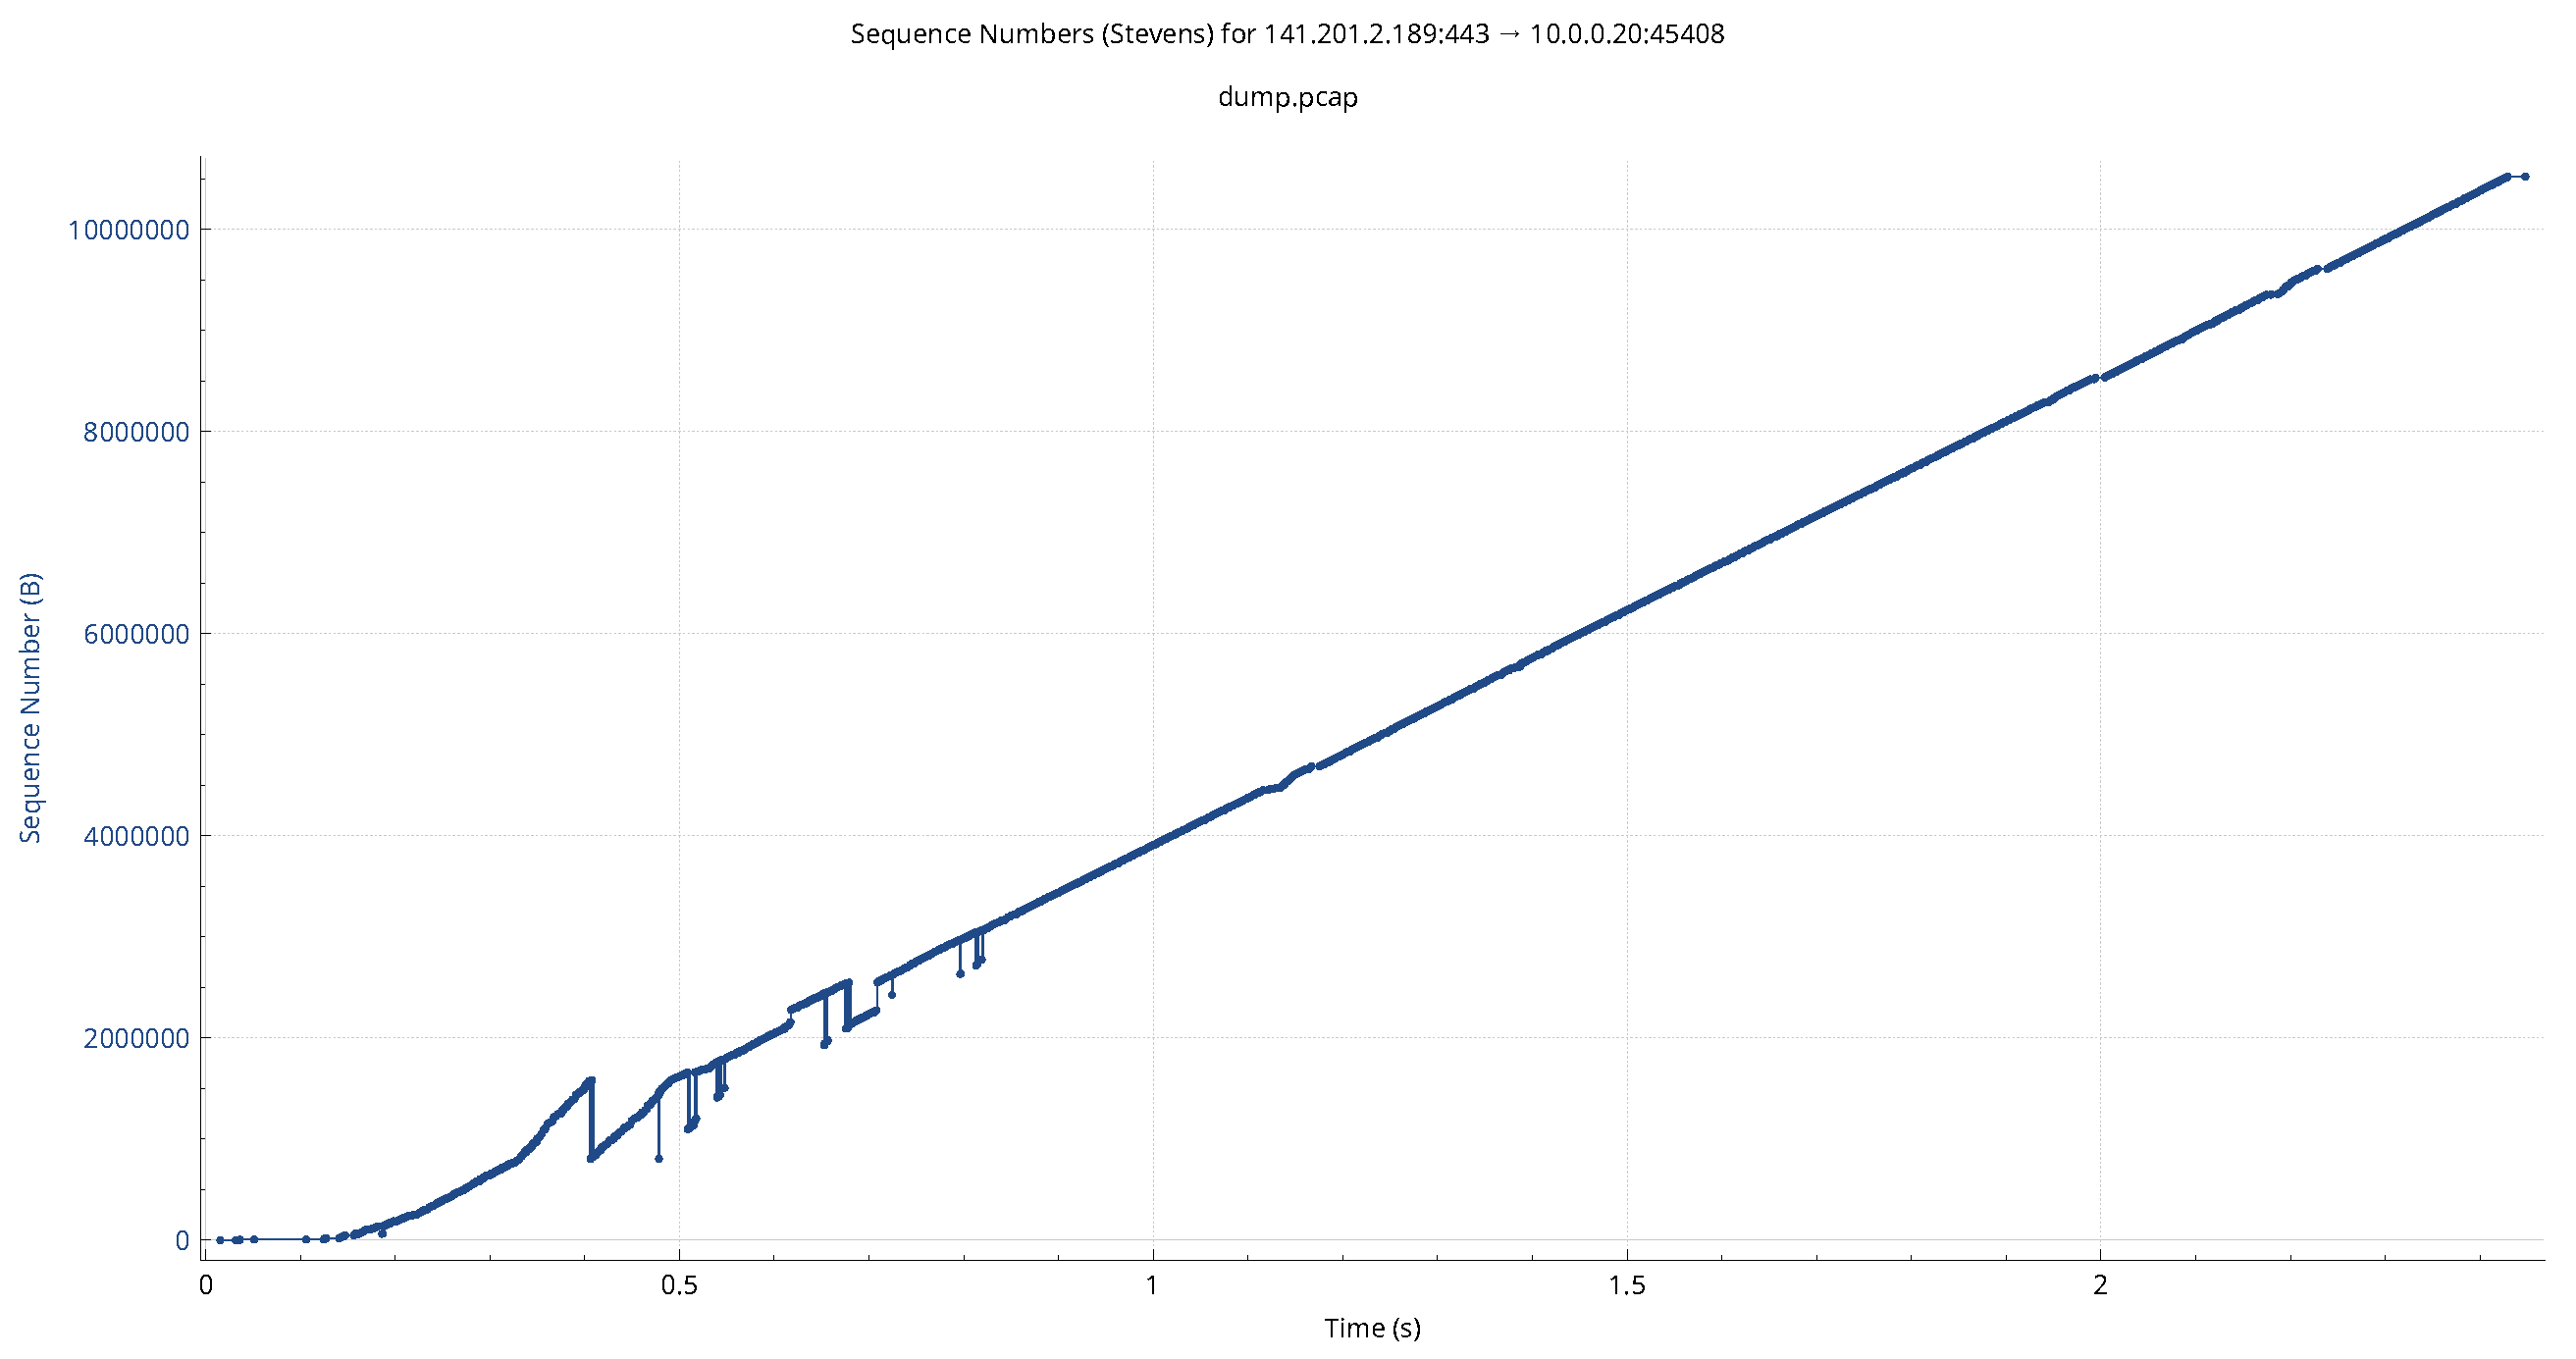
\includegraphics[width=1\textwidth]{../1/wireshark/constant5.pdf}
	\end{subfigure}
	\begin{subfigure}{0.5\textwidth}
		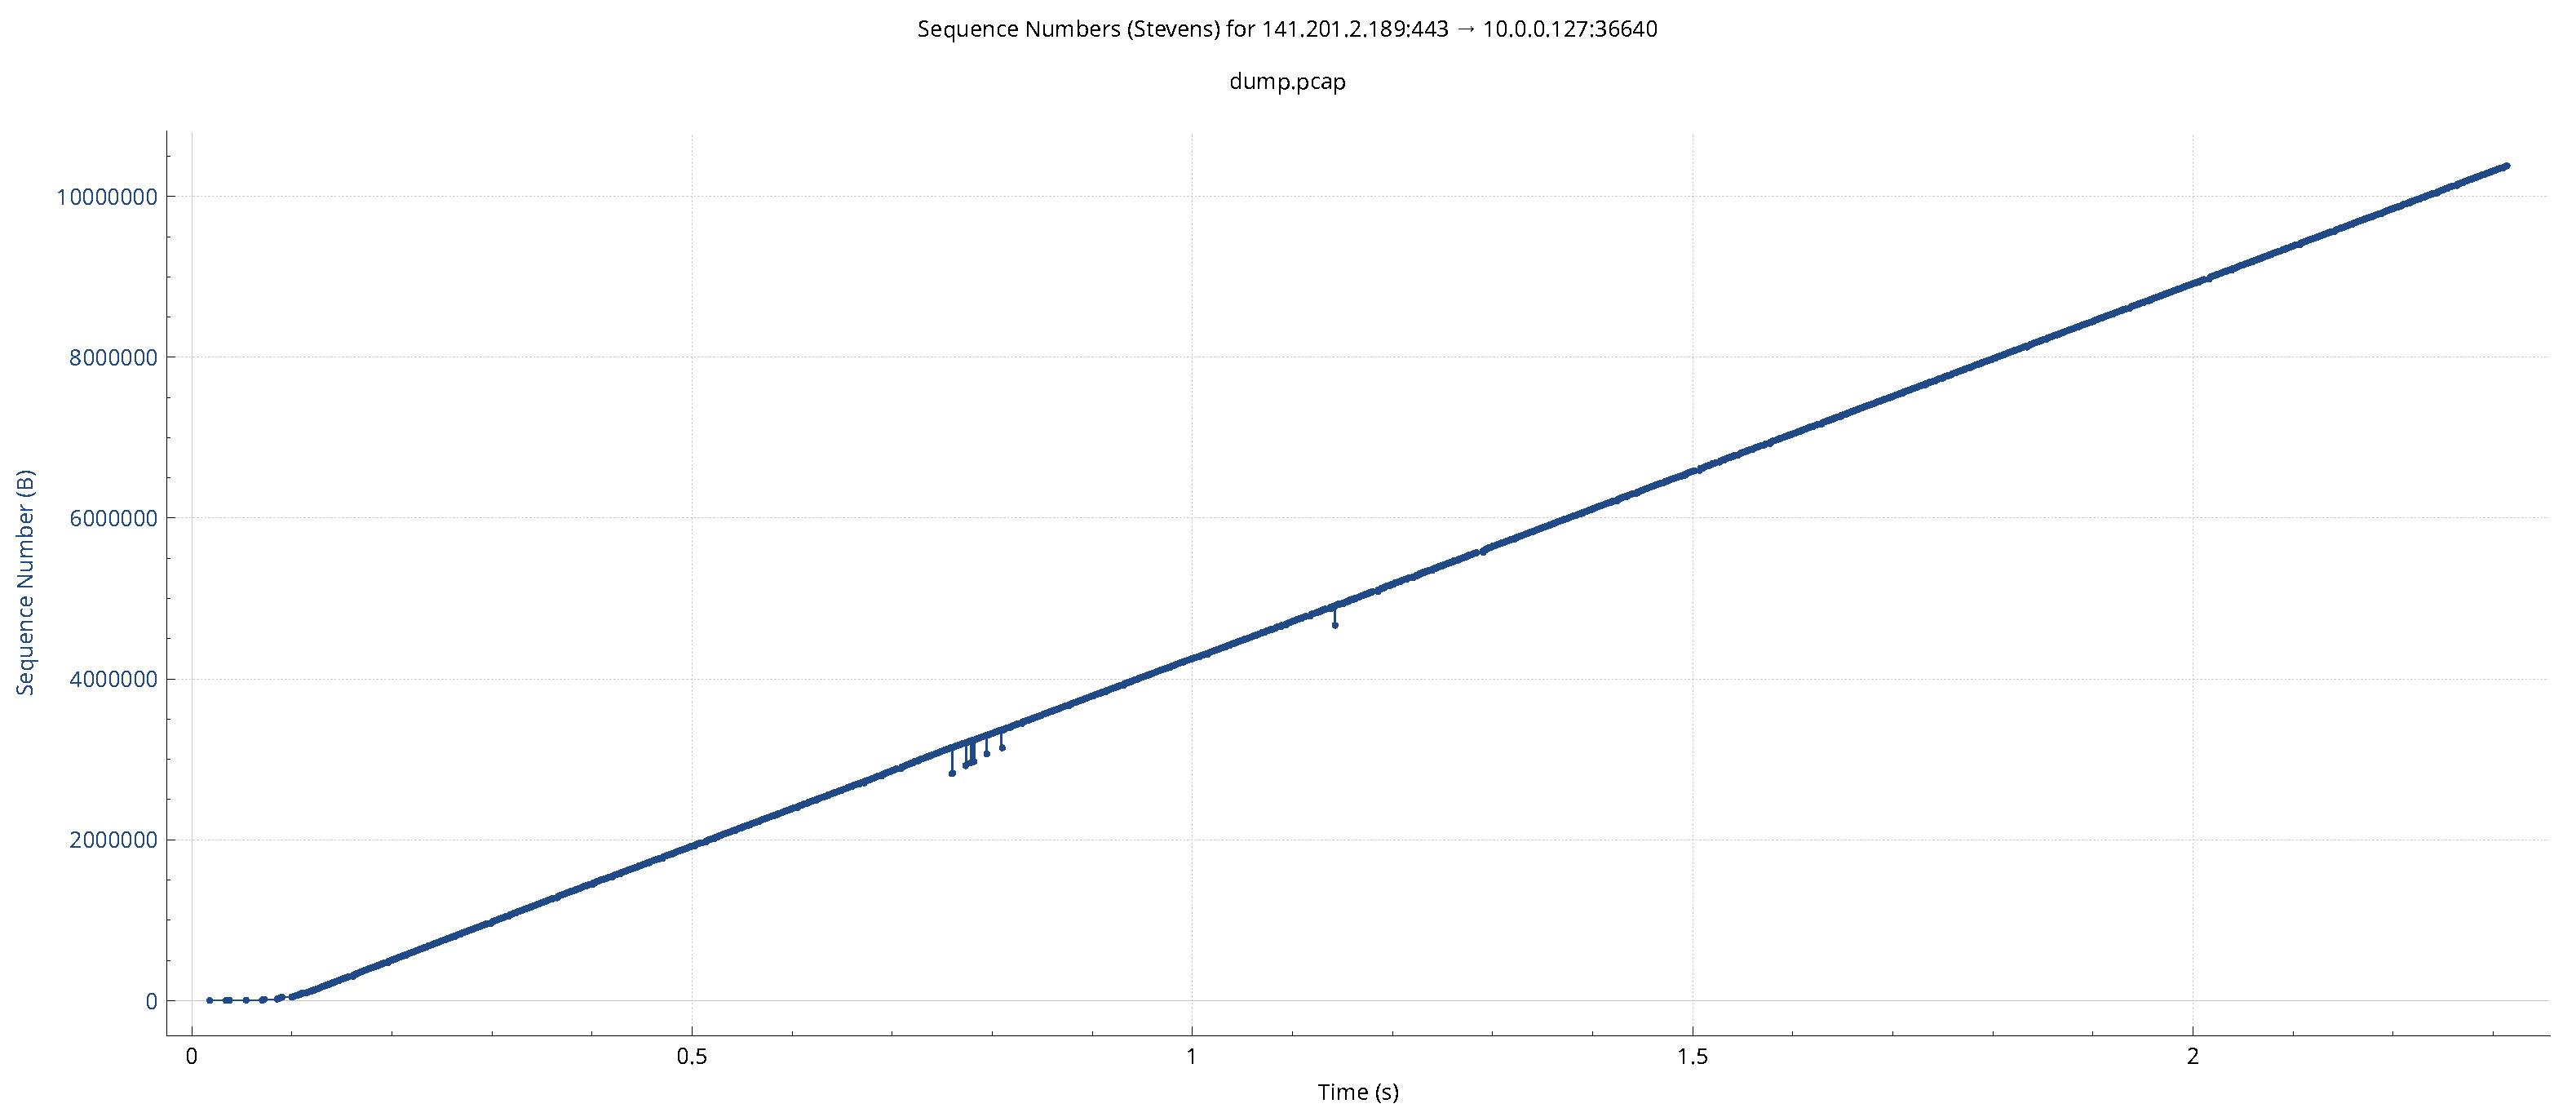
\includegraphics[width=1\textwidth]{../1/wireshark/constant6.pdf}
	\end{subfigure}
	\begin{subfigure}{0.5\textwidth}
		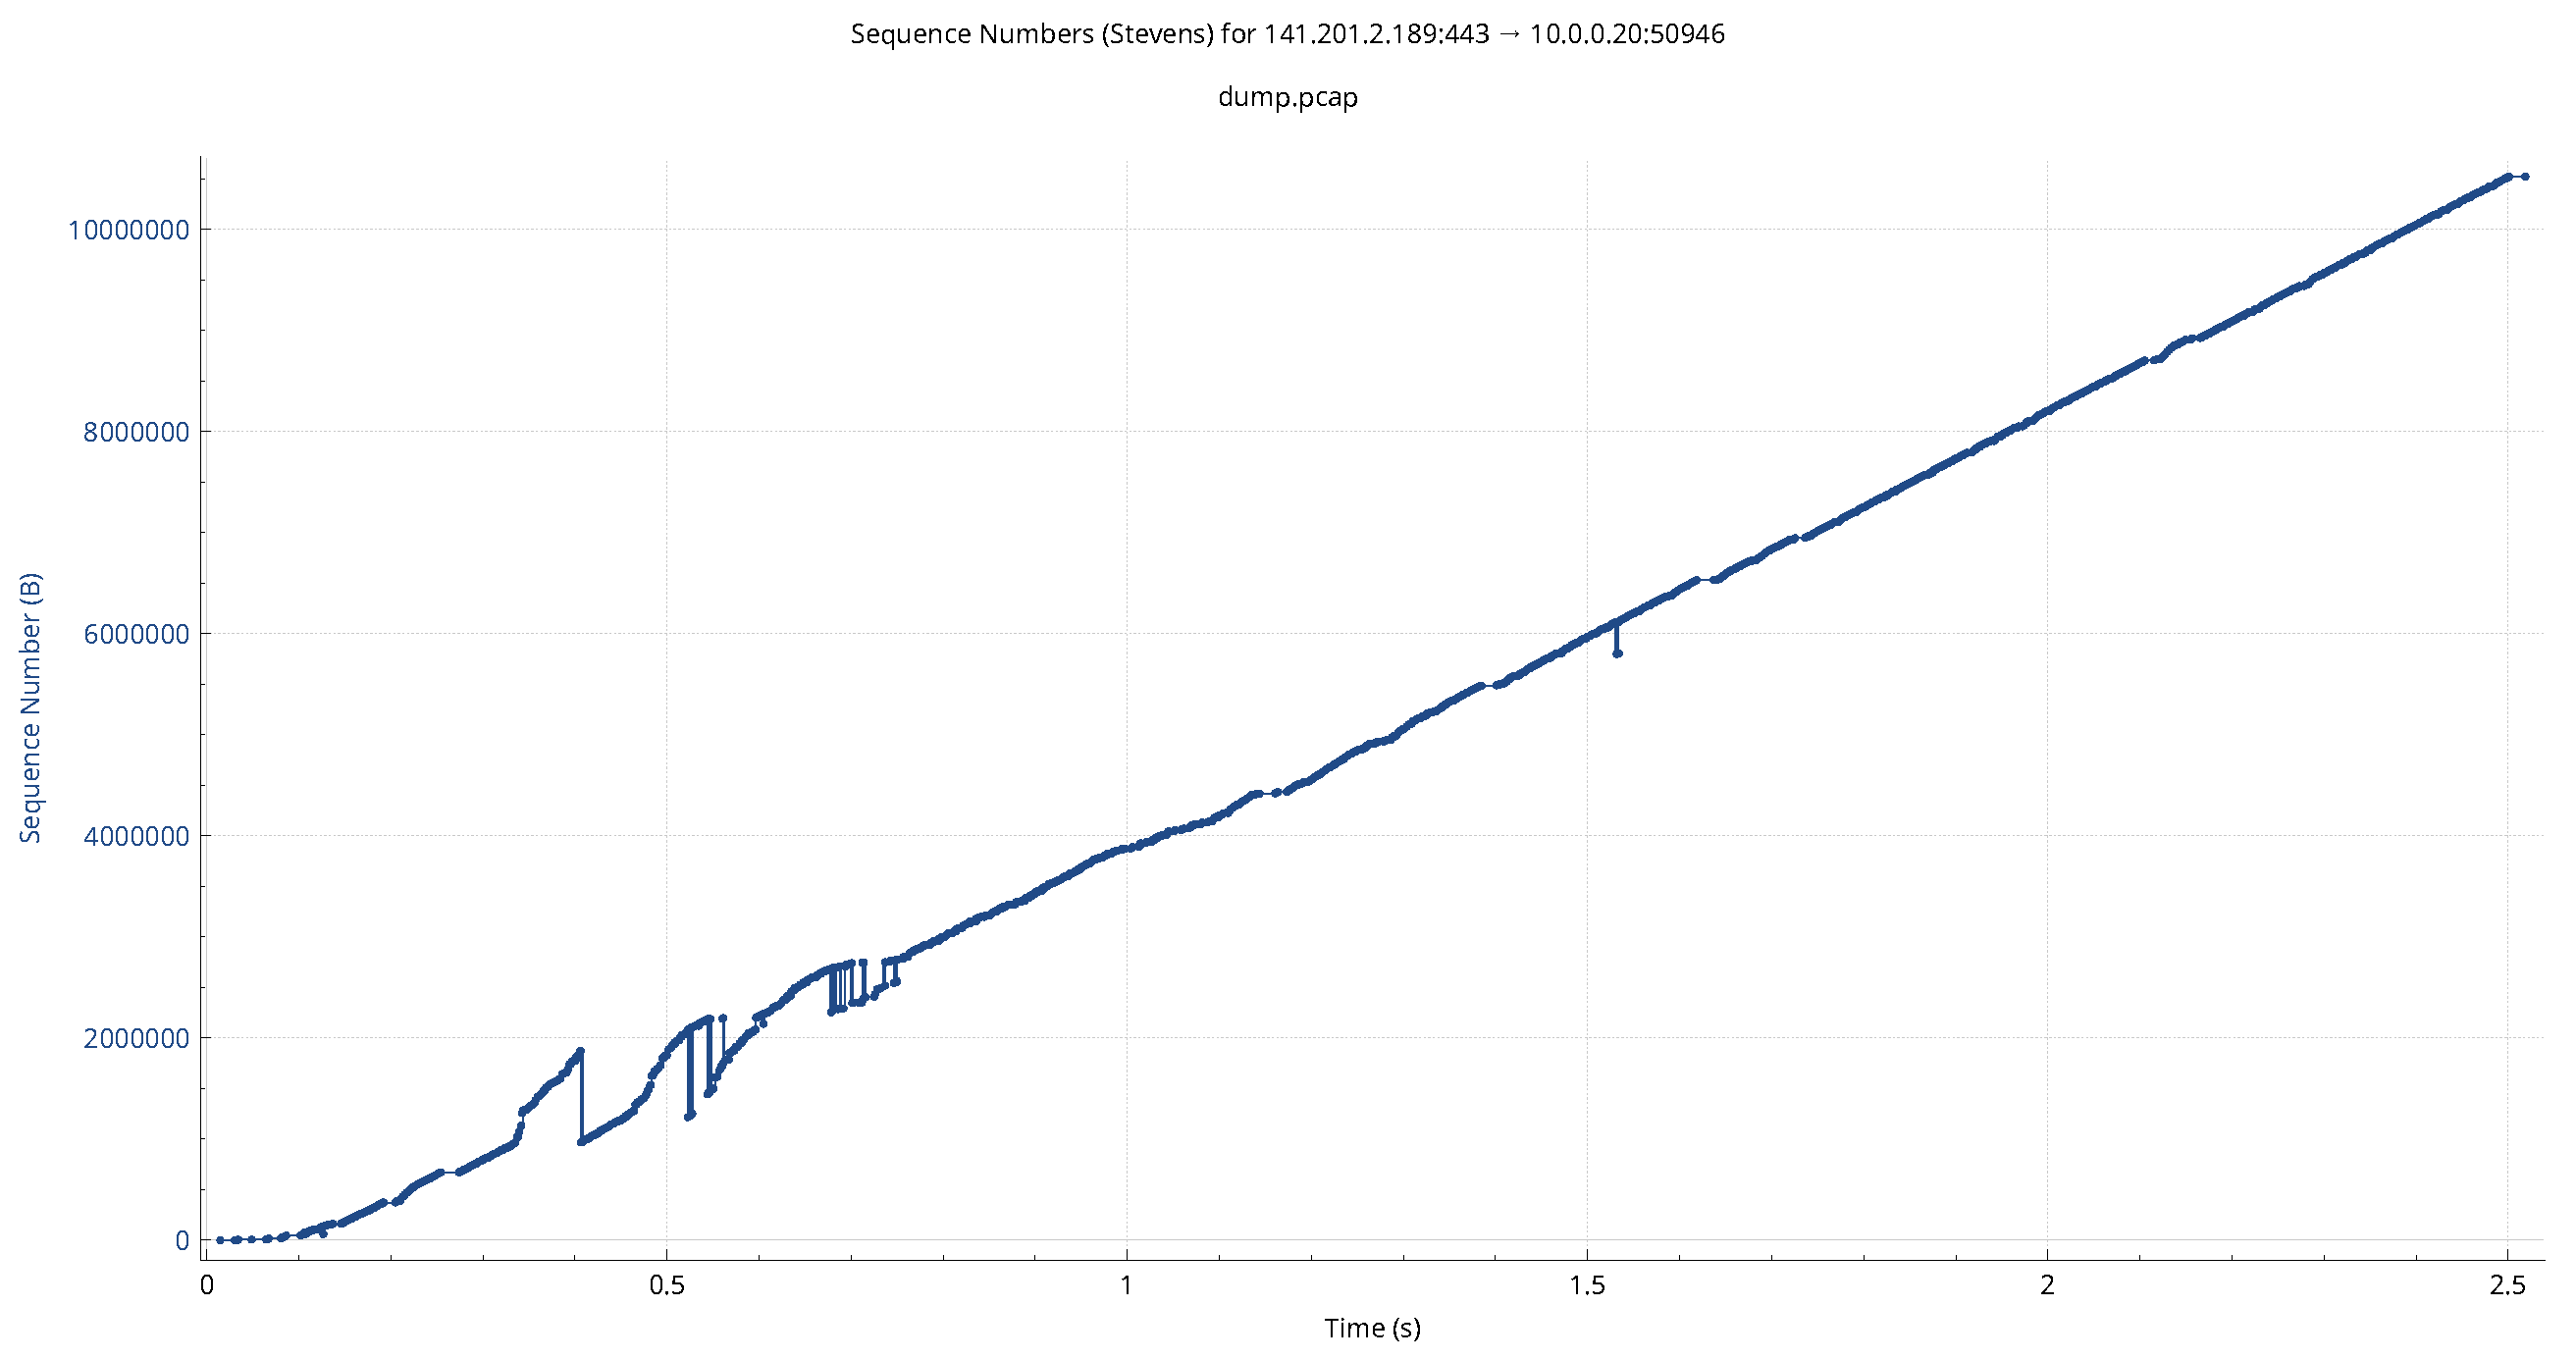
\includegraphics[width=1\textwidth]{../1/wireshark/constant7.pdf}
	\end{subfigure}
	\begin{subfigure}{0.5\textwidth}
		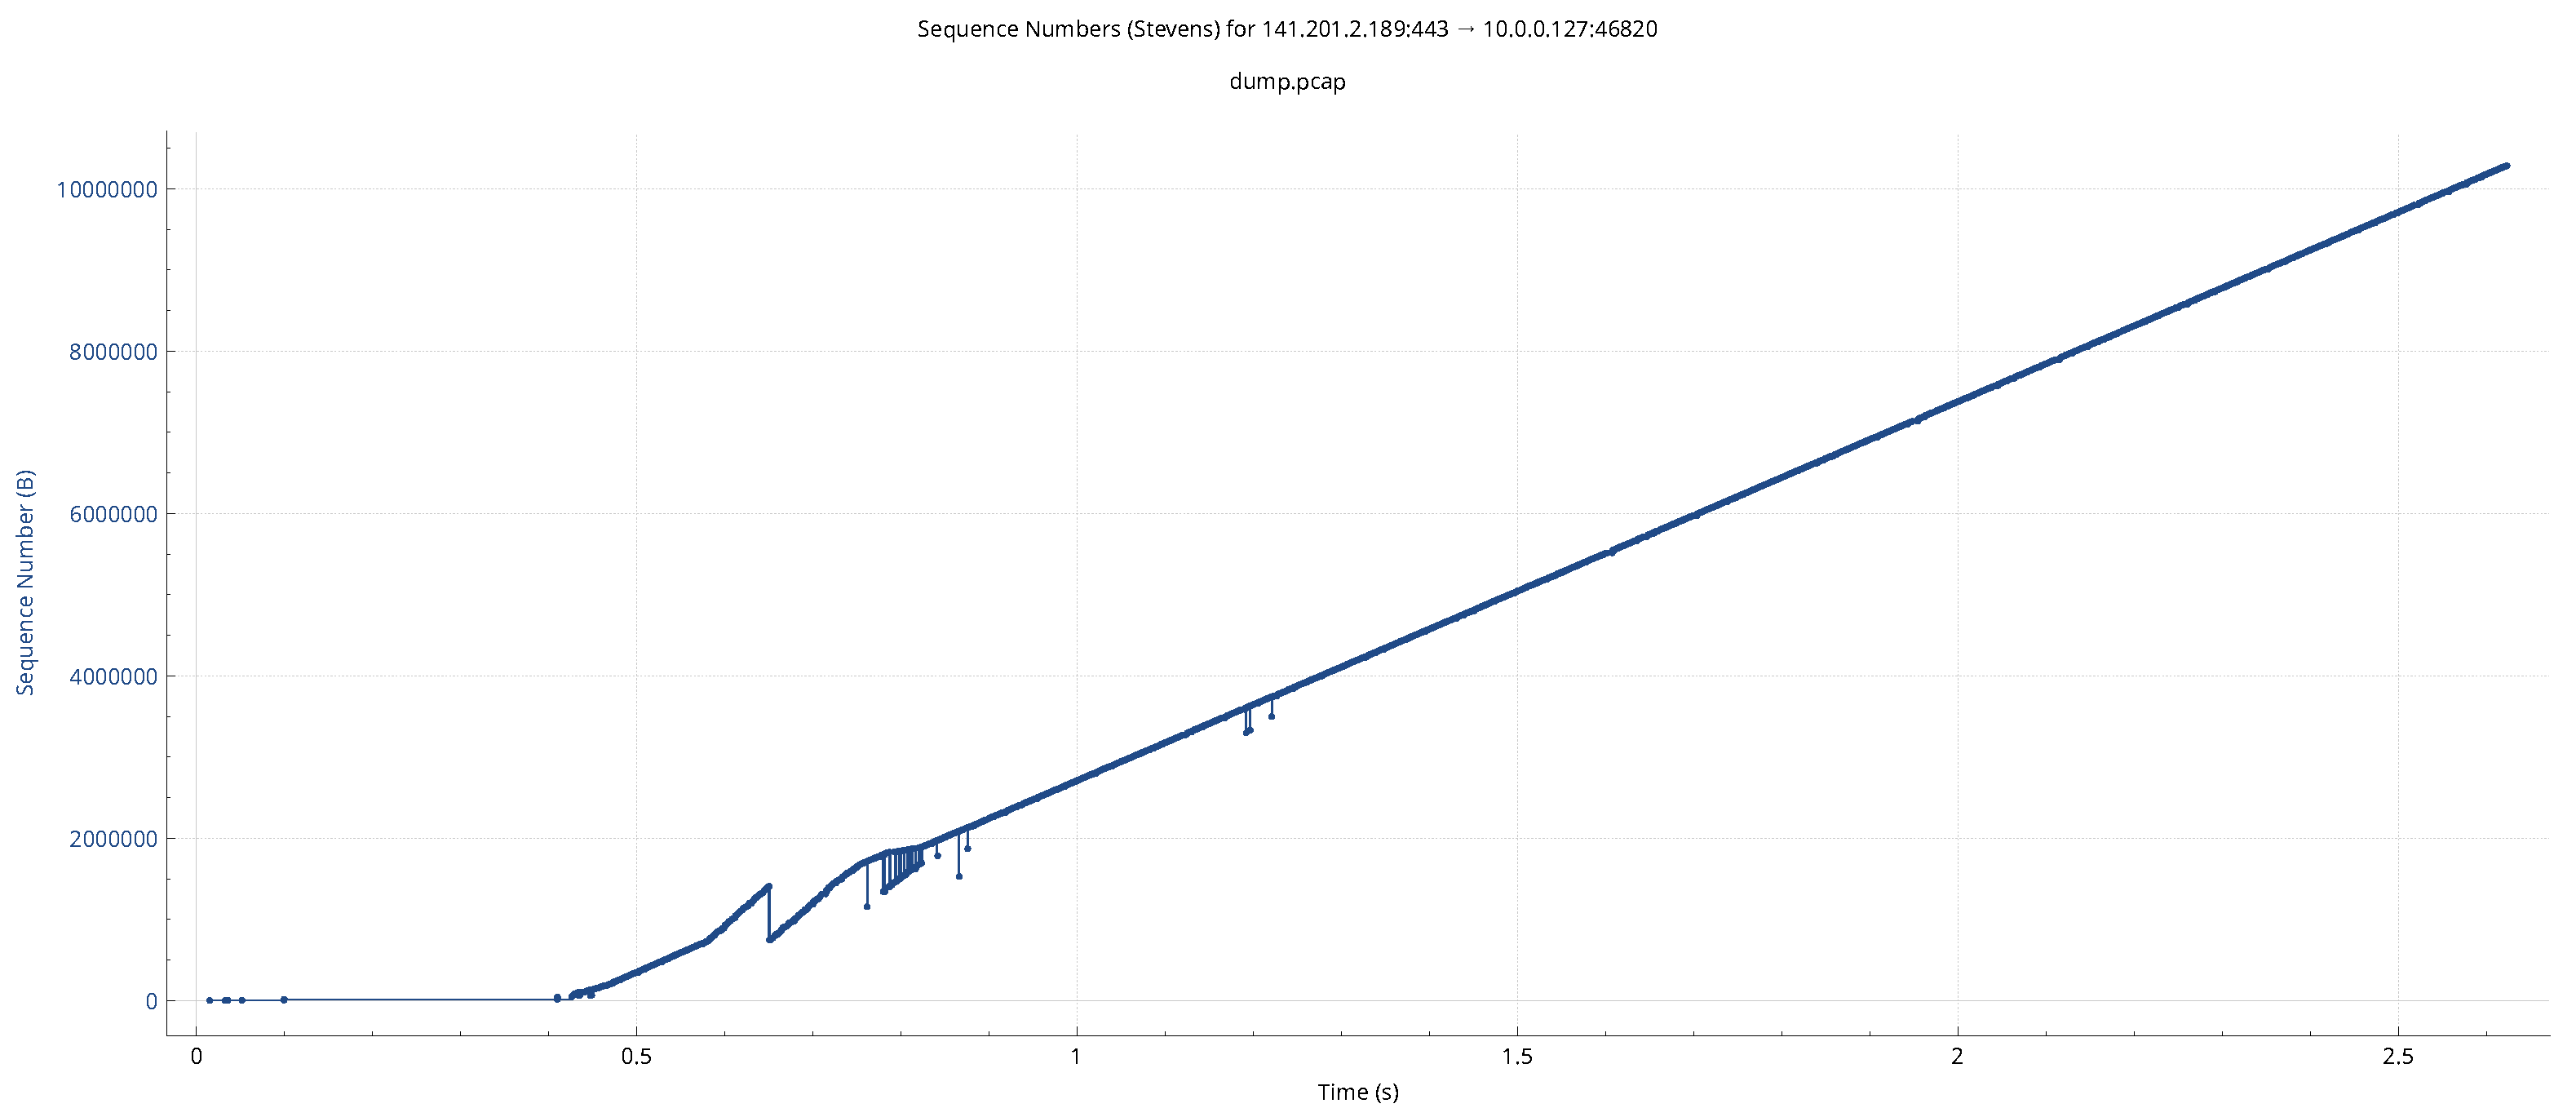
\includegraphics[width=1\textwidth]{../1/wireshark/constant8.pdf}
	\end{subfigure}
	\begin{subfigure}{0.5\textwidth}
		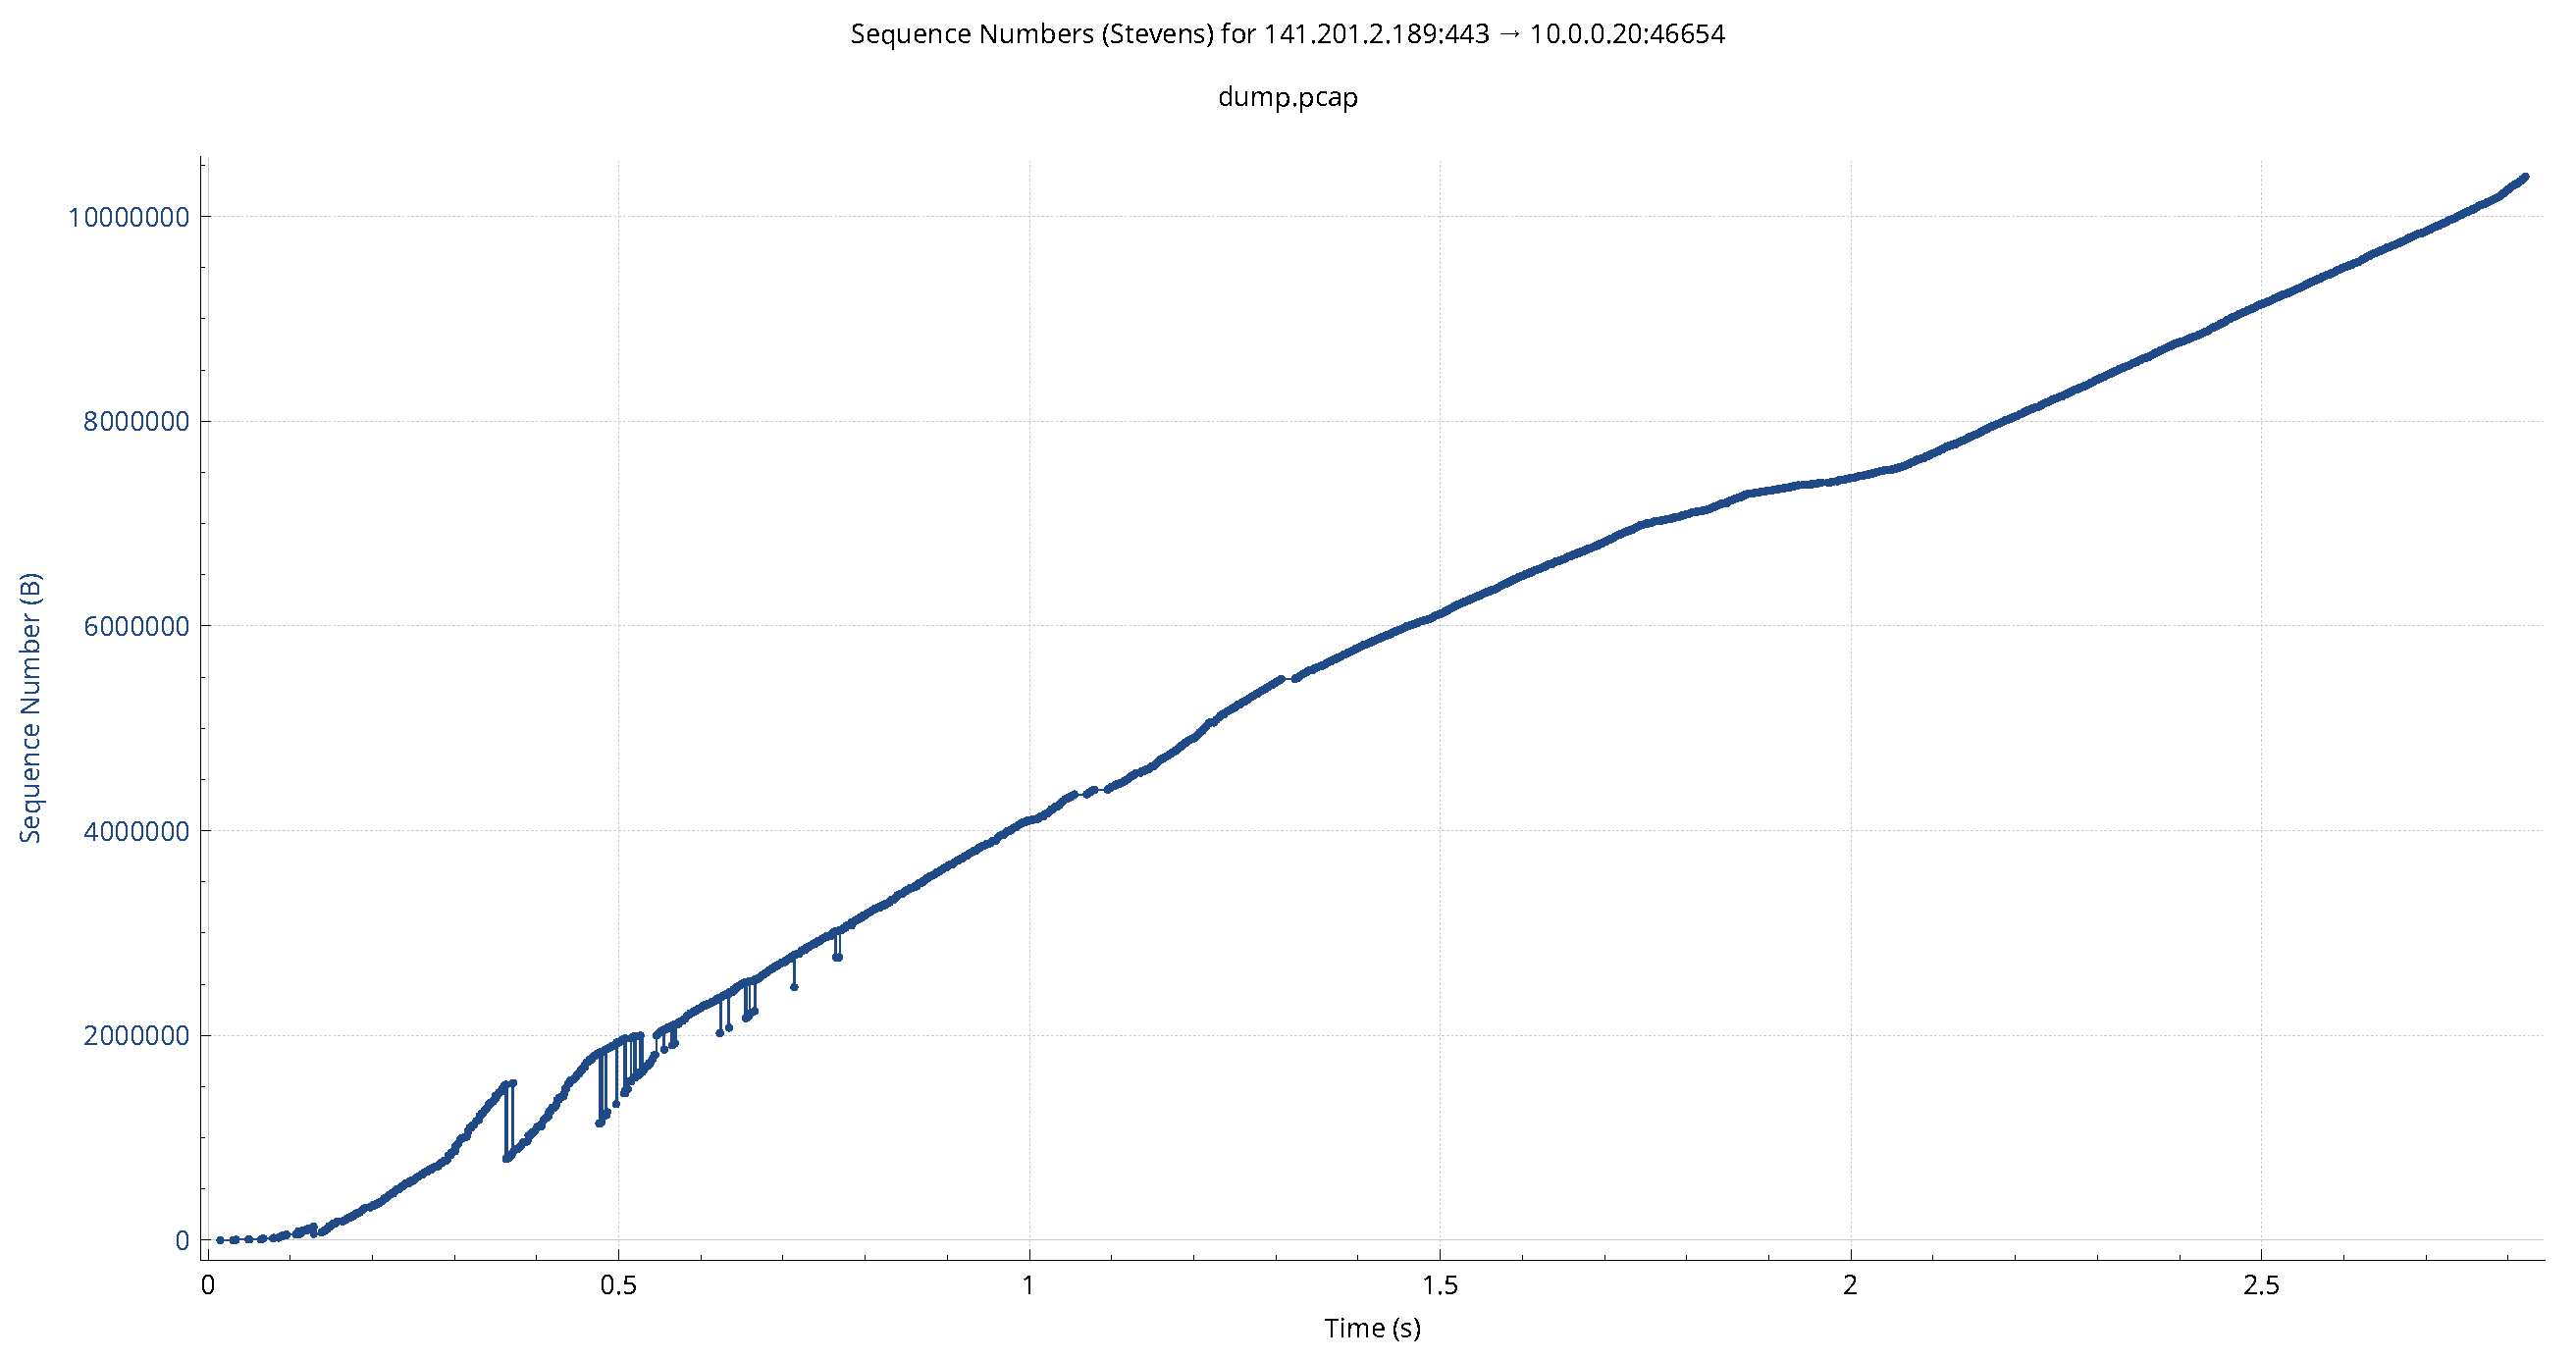
\includegraphics[width=1\textwidth]{../1/wireshark/constant9.pdf}
	\end{subfigure}
	\begin{subfigure}{0.5\textwidth}
		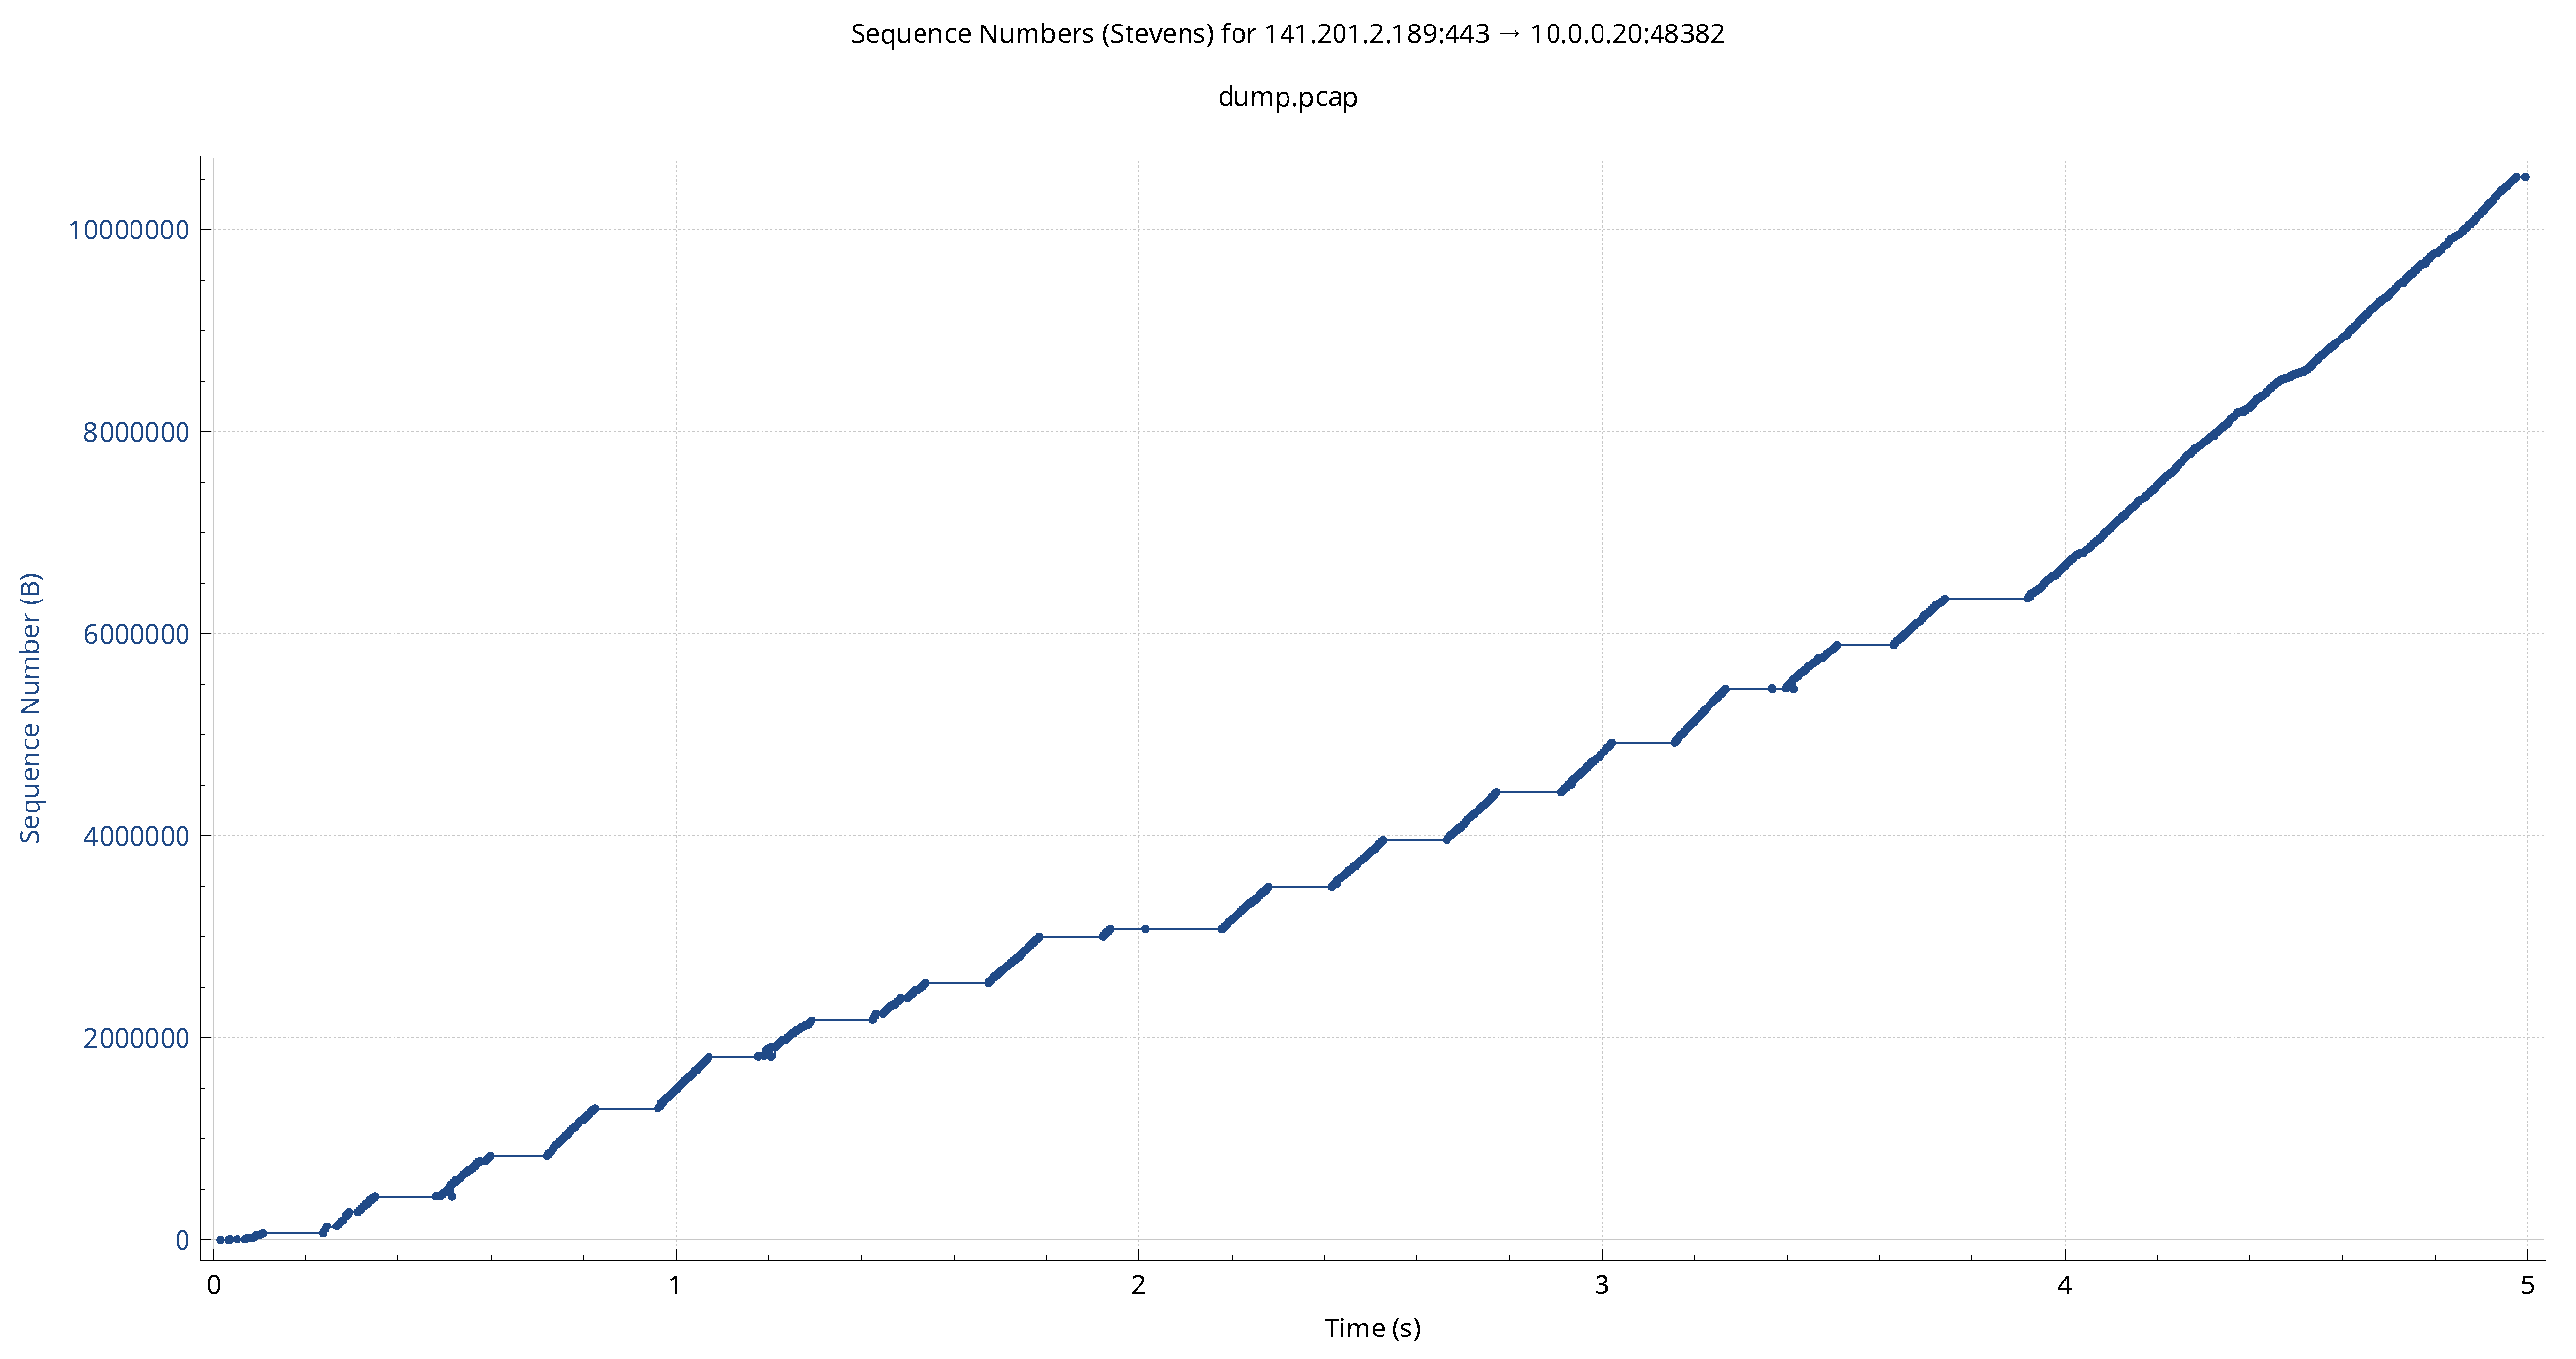
\includegraphics[width=1\textwidth]{../1/wireshark/constant10.pdf}
	\end{subfigure}
	\caption{10 Messungen bei konstanter Distanz}
\end{figure}

\section{Warum darf frau/man dabei nur den eigenen Download messen? Halten Sie sich daran!}
\vspace{5cm}%vspace

\section{Bonus 1}
\subsection{Aufgabenstellung}
\textit{Wie lässt sich die Empfangsgüte verschlechtern, ohne sich vom AP zu entfernen?}

\section{Bonus 2}
\subsection{Aufgabenstellung}
\textit{Wie kann die Aufgabe mit Linux-“Bordmitteln“ auf der commandline gelöst werden?}

\section{Zeitaufwand}
\end{document}
